\documentclass[a4paper,12pt,oldfontcommands]{abntex2}

\usepackage[num]{abntex2cite}
\usepackage[utf8]{inputenc}
\usepackage[T1]{fontenc}
\usepackage{listings}
\usepackage[most]{tcolorbox}
\tcbuselibrary{listings,breakable}
\usepackage{bchart}
\usepackage[colorinlistoftodos]{todonotes}

\citebrackets[]

% Document information

\def \myUniversity {Universidade Federal de Pernambuco}
\def \myDepartment {Centro de Informática}
\def \myGraduation {Graduação em Ciência da Computação}
\def \myTitle {Análise e implementação de estruturas de dados seguras para threads, não-bloqueantes, em Haskell}
\def \myAuthor {Paulo Vitor Julião Lieuthier}
\def \myAuthorEmail {pvjl@cin.ufpe.br}
\def \mySupervisor {Fernando Castor}
\def \mySupervisorEmail {castor@cin.ufpe.br}
\def \myCity {Recife}
\def \myDate{2017}

\autor{\myAuthor}
\titulo{\myTitle}
\data{\myDate}
\instituicao{\myUniversity}
\local{\myCity}
\tipotrabalho{Trabalho de Graduação}
\orientador{\mySupervisor}
\preambulo{Trabalho de Conclusão de Curso apresentado à Universidade Federal de Pernambuco -- UFPE, como requisito parcial para obtenção do título de Bacharel em Ciência da Computação.}

% Macros

\newtcblisting[blend into=figures]{code}[2]{
    listing options={
        style=tcblatex,
        language={Haskell}
    },
    label={#1},
    title={#2},
    listing only,
    enhanced,
    breakable
}

\newtcolorbox[blend into=figures]{graph}[2]{
    enhanced,
    title={#1},
    label={#2},
    width=.8\textwidth
}

\begin{document}

\pretextual

% Formating

\renewcommand{\arraystretch}{1.3}
\setlength{\tabcolsep}{10pt}

% Front matter and initial pages

\pagenumbering{roman}

%\begin{titlepage}
{\center%\setstretch{1.0}
\newcommand{\HRule}{\rule{\linewidth}{0.5mm}} % Defines a new command for the horizontal lines, change thickness here

 % Center everything on the page

%----------------------------------------------------------------------------------------
%	LOGO SECTION
%----------------------------------------------------------------------------------------

\begin{minipage}{\textwidth}
\center

\includegraphics[height=2.5cm]{img/logo-ufpe}
\hspace{\fill}

\includegraphics[height=2.5cm]{img/logo-cin}
\end{minipage}
\\[1.5cm]
 
%----------------------------------------------------------------------------------------
%	HEADING SECTIONS
%----------------------------------------------------------------------------------------

\textsc{\LARGE \myUniversity}\\[0.5cm] % Name of your university/college
\textsc{\Large \myDepartment}\\[0.5cm] % Major heading such as course name
\textsc{\large \myGraduation}\\[0.5cm] % Minor heading such as course title

%----------------------------------------------------------------------------------------
%	TITLE SECTION
%----------------------------------------------------------------------------------------

\HRule \\[0.4cm]
{ \huge \bfseries \myTitle \\[0.4cm] \par} % Title of your document
\HRule \\[1.5cm]
 
%----------------------------------------------------------------------------------------
%	AUTHOR SECTION
%----------------------------------------------------------------------------------------

\begin{minipage}{\textwidth}
\begin{flushleft} \large
\emph{Autor:}\\
\textsc{\myAuthor} \\
\texttt{\myAuthorEmail} \\
\end{flushleft}
\end{minipage}

\begin{minipage}{\textwidth}
\begin{flushright} \large \vspace{0.5cm}
\emph{Orientador:} \\
\textsc{\mySupervisor} \\
\texttt{\mySupervisorEmail}
\end{flushright}
\end{minipage}

%----------------------------------------------------------------------------------------
%	DATE SECTION
%----------------------------------------------------------------------------------------

\vfill
{\large \myCity, \myDate}
 
%----------------------------------------------------------------------------------------
}
%\end{titlepage}


\cleardoublepage

\imprimirfolhaderosto

\begin{folhadeaprovacao}
    \begin{center}
        {\ABNTEXchapterfont\large\imprimirautor}
        \vspace*{\fill}\vspace*{\fill}
        \begin{center}
            \ABNTEXchapterfont\bfseries\Large\imprimirtitulo
        \end{center}
        \vspace*{\fill}
        \hspace{.45\textwidth}
        \begin{minipage}{.5\textwidth}
            \imprimirpreambulo
        \end{minipage}%
        \vspace*{\fill}
    \end{center}
    Trabalho aprovado. \imprimirlocal, 12 de dezembro de 2017:
    \assinatura{\textbf{Prof. \imprimirorientador} \\ Orientador}
    \assinatura{\textbf{Prof. Fernando Castor} \\ Avaliador}
    \begin{center}
        \vspace*{0.5cm}
        {\large\imprimirlocal}
        \par
        {\large\imprimirdata}
        \vspace*{1cm}
    \end{center}
\end{folhadeaprovacao}

\begin{dedicatoria}
     \vspace*{\fill}
     \begin{flushright}
         Soli Deo Gloria
     \end{flushright}
     \vspace*{\fill}
\end{dedicatoria}

\begin{agradecimentos}
    \vspace*{\fill}
    \begin{flushright}
        Agradeço aos meus pais, irmãos e amigos que me apoiaram e me incentivaram durante toda a graduação e a produção desse trabalho. Agradeço especialmente ao meu professor orientador, pela incrível paciência e confiança.
        \\\vspace*{0.5cm}
        Por último, expresso minha profunda gratidão à minha esposa, sem a qual terminar esse trabalho teria sido simplesmente impossível para mim. Dani, ``muitas mulheres são exemplares, mas você a todas supera''!
    \end{flushright}
    \vspace*{\fill}
\end{agradecimentos}

\begin{resumo}
    Apesar de desejáveis em alguns cenários, algoritmos bloqueantes podem causar grandes penalidades de performance, especialmente com a ocorrência de contenção de travas (lock contention). Alternativas ao uso de travas explícitas têm sido sugeridas, como o controle de concorrência otimista (utilizando, por exemplo, memória transacional). Naturalmente, existe desvatagens em todas as alternativas, como a baixa eficiência na pararelização das tarefas.   O   objetivo   desse   trabalho   é   implementar,  em   Haskell,   estruturas   de   dados concorrentes seguras para threads e não-bloqueantes, que são uma outra alternativa. A desvantagem nesse caso é a alta complexidade de implementação e a maior frequência de problemas sutis. Para satisfazer as propriedades de segurança e de não-travamento, instruções de máquina CAS (\textit{compare-and-swap}) e memória transacional foram utilizadas.
    \hfill\break
    \hfill\break
    \noindent
    \textbf{Palavras-chave}: Haskell; concorrência; paralelismo; estruturas de dados; lock contention; compare-and-swap;
\end{resumo}

\begin{resumo}[Abstract]
Although desirable in some scenarios, blocking algorithms may cause tremendous performance penalties, specially in occurrence of lock contention. Alternatives to the use of explict locks have been suggested, like optimistic concurrency control (using, for instance, transactional memory). Naturally, there are disadvantages in all alternatives, like low efficiency in the parallelization of tasks. The goal of this work is to implement, in Haskell, thread-safe, non-blocking data structures, which are another alternative. The disadvantage in this case é the high implementation complexity and the more often occurrence of subtle issues. To satisfy the safety and non-blocking properties, CAS (compare-and-swap) machine instructions and transacional memory were used.
    \hfill\break
    \hfill\break
    \noindent
    \textbf{Keywords}: Haskell; concurrency; parallelism; data structures; lock contention; compare-and-swap;
\end{resumo}

\cleardoublepage

\tableofcontents

% Document content

\textual
\pagenumbering{arabic}

\chapter{Introdução}

Com a popularização de dispositivos de computação portáteis e a crescente dificuldade com os limites físicos de tamanho dos semicondutores, a corrida pela maior frequência de operação dos processadores perdeu sentido. Dispositivos portáteis dependem de fontes de energia limitadas, e alta frequência de processadores levam ao alto consumo de energia e dissipação de calor \cite{schone2012memory}.

A solução encontrada foi a fabricação de processadores multinúcleo, componentes de computação com duas ou mais unidades de processamento que funcionam paralela e independentemente \cite{kataoka2015power}. Esse paralelismo, contudo, não é trivialmente aproveitável. O processo de desenvolvimento do software precisa levar em conta a capacidade de paralelização dos componentes de hardware \cite{hoare1972towards}.  
A complicação de tal tarefa se deve principalmente à necessidade de sincronização de tarefas paralelas ou concorrentes: duas unidades de processamento podem ser programadas para fazer uso de um mesmo espaço de memória, potencialmente executadas sobrepostas. Essa sobreposição (interleaving) pode causar inconsistências no valor contido no espaço de memória sendo compartilhado, gerando problemas de sincronização e comportamentos inesperados.

Pesquisa extensiva tem sido feita para encontrar soluções para problemas de sincronização. A solução mais comum é o uso de monitores (locks) para forçar a sequencialização do acesso à porções da memória compartilhada, chamadas de regiões críticas \cite{tallent2010analyzing}. O uso de monitores não é trivial, e o descuido leva a bugs difíceis de identificar e reproduzir, assim como deadlocks.

Além disso, o uso de travamento para sincronização pode acarretar alto custo de performance, especialmente quando muitas tarefas concorrentes são programadas para fazer uso da mesma região crítica, o que é chamado de contenção (lock contention) \cite{tallent2010analyzing}. Com a evolução dos componentes de hardware, processadores modernos são capazes de executar instruções já levando em consideração a execução de componentes de software paralelos ou concorrentes. Instruções atômicas podem ser utilizadas para desenvolver programas concorrentes seguros sem o custo de performance do uso de travamento, apesar de aumentar ainda mais a complexidade de implementação \cite{michael1998nonblocking}.

Uma vez que estruturas de dados são componentes fundamentais no desenvolvimento de software, existem muitas implementações de estruturas de dados concorrentes e paralelas. Contudo, há ainda relativamente poucos resultados de implementações não-bloqueantes.

No capítulo \ref{chapter-haskell-primer}, é feito um sobrevôo sobre a linguagem Haskell e suas estruturas de suporte à concorrência. O capítulo \ref{chapter-data-structures} trata da problemátca do uso de estruturas de dados por múltiplas threads e um possível passo-a-passo para alcançar uma implementação que seja segura para threads e sem travamento. O capítulo \ref{chapter-implementation} apresenta uma análise de cada implementação e o capítulo \ref{chapter-analysis} uma análise dos resultados obtidos.

\chapter{Concorrência e paralelismo em Haskell}\label{chapter-haskell-primer}

\section{A Linguagem Haskell}

Haskell é uma linguagem de propósito geral, puramente funcional e de avaliação não-estrita. Contém funcionalidades como tipos de dados abstratos, casamento de padrões, compreensão de listas, polimorfismo paramétrico, funções de alta ordem, \textit{currying} e \textit{higher-kinded types} \cite{jones2003haskell}.

Por ser uma linguagem ``pura'', Haskell impõe, por padrão, transparência referencial. Isso significa que, por padrão, uma função em Haskell aplicada a seus argumentos sempre retornará o mesmo resultado, o que permite que otimizações sejam feitas transparentemente pelo compilador (como, por exemplo, memoização) \cite{brown2007monadic}.

Haskell é populamente conhecida como uma linguagem preguiçosa (\textit{lazy}), embora o termo mais exato seja não-estrita \cite{hudak2007history}. \textit{Lazyness} é apenas uma técnica de implementação de linguagens não-estritas, onde a avaliação de uma expressão é feita apenas quando o seu resultado se faz necessário. Haskell, de fato, não é uma liguagem puramente preguiçosa: casamento de padrões, a primitiva \texttt{seq} e otimizações internas do compilador impõem avaliação estrita.

\section{Estruturas de dados em Haskell}

A implementação padrão e uso de listas em Haskell é feita usando apenas construtores (Figura \ref{list-definition}) e casamento de padrões (Figura \ref{pattern-match-usage}).

\begin{code}{list-definition}{Definição do tipo \texttt{List} \cite{jones2003haskell}}
data [a] =  [] | a : [a] deriving (Eq, Ord)
\end{code}

\begin{code}{pattern-match-usage}{Implementação da função \texttt{dropWhile}, usando casamento de padrões}
dropWhile :: (a -> Bool) -> [a] -> [a]
dropWhile _ []          =  []
dropWhile p xs@(x:xs')
            | p x       =  dropWhile p xs'
            | otherwise =  xs
\end{code}

A implementação a ser apresentada nesse trabalho, entretanto, faz uso de ponteiros, com o tipo \texttt{IORef}. Isso é necessário para fazer uso das operações \textit{compare-and-swap}.

Essa característica representa um grande déficit de usabilidade, se comparada às listas nativas de Haskell. Porém, como toda aplicação em Haskell precisa de uma ação monádica \texttt{IO} para ser executada (e, assim, produzir efeitos colaterais), é de se imaginar que esse é um preço pequeno tendo em vista os benefícios.

\section{Concorrência e paralelismo em Haskell}

A implementação convencional de Haskell, o compilador GHC (Glasgow Haskell Compiler), fornece várias primitivas para alcançar concorrência e paralelismo em Haskell. Essas primitivas são definidas em extensões da especificação original de Haskell, como Concurrent Haskell \cite{jones1996concurrent} e STM (Software Transaction Memory) \cite{harris2005composable}, entre outros.

\subsection{Concurrent Haskell}

Concurrent Haskell define um tipo básico de sincronização: \texttt{type MVar a}.

Um valor do tipo \texttt{MVar t} representa uma região mutável da memória que pode estar vazia ou conter um valor do tipo \texttt{t} \cite{jones1996concurrent}. São definidas também operações primitivas:

\begin{description}
    \item [\texttt{newMVar :: IO (MVar a)}.] Cria um novo \texttt{MVar}.
    \item [\texttt{takeMVar :: MVar a -> IO a}.] Bloqueia a thread atual até que o valor esteja não-vazio, e então extrai o valor para ser retornado, e esvazia o \texttt{MVar}.
    \item [\texttt{putMVar :: MVar a -> a -> IO ()}.] Bloqueia a thread atual até que o valor esteja vazio, e então escreve o parâmetro no valor.
    \item [\texttt{forkIO :: IO ()}.] Inicia uma nova thread, administrada pelo sistema de execução do GHC (thread leve).
\end{description}

Por causa da avaliação não-estrita de Haskell, a operação \texttt{forkIO} requer um mecanismo de sincronização, como \texttt{MVar}. Isso porque se algum valor da thread principal que ainda não foi totalmente avaliado for acessado na nova thread, seria necessário sincronização no avaliador \cite{jones1996concurrent}. Por isso, toda comunicação entre threads deve ser feita \texttt{MVars} (ou outros mecanismos de sincronização).

O tipo \texttt{MVar} pode funcionar como variável mutável (segura para threads), como canal de elemento único (onde \texttt{putMVar} funcionaria como send, e \texttt{takeMVar} como receive, respectivamente) ou como semáforo binário, simplesmente para sincronização \cite{jones1996concurrent}.
Existem outras construções de concorrência definidas no Concurrent Haskell, mas todas são construídas sobre a primitiva \texttt{MVar}.

\subsection{Haskell STM (Software Transaction Memory)}

Um problema das primitivas de sincronização do Concurrent Haskell, além da complexidade de implementação, é a falta de \textit{composability} (componibilidade) \cite{harris2005composable}. Ou seja, se faz necessário conhecer detalhes de implementação para construir abstrações de concorrência maiores a partir de abstrações menores \cite{harris2005composable}.

A extensão STM permite a construção de programas concorrentes utilizando o conceito de transações, que podem ser reexecutadas caso falhem. Para permitir isso, transações não podem conter ações que modifiquem o estado global do programa (ações \texttt{IO}). Portanto, as transações são modeladas por um tipo específico, e junto à capacidade de reexecutá-las, isso permite a construção de abstrações independentemente dos detalhes de implementação.

Semelhantemente ao Concurrent Haskell, Haskell STM define um tipo para representar um valor mutável seguro para threads, \texttt{TVar a}, juntamente com as operações \texttt{newTVar}, \texttt{readTVar} e \texttt{writeTVar}, análogas às do tipo \texttt{MVar}. Não é necessário que as operações sejam bloqueantes, basta que a transação seja reexecutada caso os valores utilizados tenham sido alterados por outra thread.

Há também outras operações:

\begin{description}
\item [\texttt{atomically :: STM a -> IO a}.] Recebe uma transação e retorna uma ação IO que, quando executada, executa a transação atomicamente com respeito a todas as outras transações que usem as mesmas \texttt{TVar}s.
\item [\texttt{retry :: STM a}.] Aborta a transação, descartando todos os possíveis efeitos, e a reinicia. Pode ser usada para implementar algoritmos bloqueantes.
\item [\texttt{orElse :: STM a -> STM a -> STM a}.] Permite componibilidade trivial de transações como alternativas, de modo que se a primeira for abortada, a segunda é executada.
\end{description}

A implementação da STM segue o princípio da concorrência otimista, ou seja, supõe-se que a maioria das transações serão concluídas com sucesso, sem serem invalidadas. Caso na execução de um determinado programa a quantidade de conflitos entre transações seja alto, a performance será degradada, podendo ser pior do que o programa sequencial \cite{sulzmann2009comparing}.

\subsection{atomicModifyIORef}\label{subsection-atomicmodifyioref}

Outra primitiva de sincronização fornecida pelo GHC é a função \texttt{atomicModifyIORef}, que curiosamente não tem uma origem clara \cite{sulzmann2009comparing}. Ela faz parte da API do tipo \texttt{IORef}, que define um região de memória mutável, com operações não-bloqueantes a serem executadas em ações \texttt{IO} (\texttt{newIORef}, \texttt{readIORef} e \texttt{writeIORef}, análogas às do tipo \texttt{MVar}).

\texttt{IORef} pode ser visto como algo mais próximo do que é chamado em outras linguagens (e.g. C, C++) de ponteiros, ou seja, identificadores de posições de memória contendo determinados valores. A questão é que a maioria das linguagens não fornece garantias de ordenamento de operações de memória, por questões de performance \cite{herlihy2011art}. Por exemplo, a atribuição de uma posição a um ponteiro pode acontecer antes mesmo da alocação da memória no endereço proposto.

Além das linguagens, arquitetura de processadores também podem não garantir consistência sequencial, como a documentação \footnote{https://hackage.haskell.org/package/base-4.10.0.0/docs/Data-IORef.html} das operações sobre \texttt{IORef} deixa claro:

\begin{quote}
In a concurrent program, \texttt{IORef} operations may appear out-of-order to another thread, depending on the memory model of the underlying processor architecture. For example, on x86, loads can move ahead of stores.
\end{quote}

Essa característica dificulta o uso de ponteiros sem mecanismos de sincronização por mais de uma thread. Para resolver esse problema, o GHC faz uso de barreiras de memória (\textit{memory barriers}), um instrumento bastante baixo-nível para sincronização de operações de memória \cite{sulzmann2009comparing}. Isso garante consistência sequencial para determinadas operações, isto é, a garantia que o resultado das operações é o mesmo do resultado das operações se executas sequencialmente \cite{herlihy2011art}.

Em geral, essa garantia tem um custo considerado proibitivo para algumas linguagens, como Java, por inibir otimizações do compilador \cite{herlihy2011art}. Contudo, estudos recentes demonstram que o custo de adicionar barreiras de memória em todas as operações de leitura e escrita de \texttt{IORef}s é desprezível \cite{vollmer2017sc}.

Consistência sequencial ainda não é suficiente para permitir a construção da maioria dos algoritmos concorrentes. Uma operação do tipo \textit{compare-and-swap} é necessária \cite{sulzmann2009comparing}. Isso porque, mesmo com consistência sequencial, uma operação de atualização (leitura seguida de escrita) ainda precisará de sincronização.

\begin{description}
\item [\texttt{atomicModifyIORef :: IORef a -> (a -> (a, b)) -> IO b}.] Escreve, atomicamente, o primeiro valor resultante da aplicação da função ao valor atual na memória.
\end{description}

Essa operação pode ser usada para construir a operação \textit{compare-and-swap}, que é suficiente para construir vários tipos de estruturas de dados seguras para threads e não-bloqueantes \cite{valois1995lock}.

A implementação da operação \texttt{atomicModifyIORef} no GHC é semelhante ao que se apresenta na Figura \ref{atomic-ioref}.

\begin{code}{atomic-ioref}{atomicModifyIORef}
atomicModifyIORef pointer function = do
    value <- readIORef pointer
    let (newValue, result) = function value
    writeIORef pointer newValue
    return result
\end{code}

Com a exceção de que a chamada à \texttt{writeIORef} é substituída por uma operação \textit{compare-and-swap} \cite{sulzmann2009comparing}, que só escreve o novo valor se o valor antigo for igual ao valor obtido na leitura (ou seja, outra thread não o invalidou). Se o valor já fora invalidado, então a operação é reexecutada. Essa operação assemelha-se a uma mini-transação STM, sobre um único valor.

\chapter{Estruturas de dados para multiprocessadores}\label{chapter-data-structures}

Existem várias abordagens para construir estruturas de dados seguras para threads. A abordagem mais direta é usando travas. Neste trabalho, será aprecentada uma implementação de lista ligada livre de travas, construída a partir de uma solução mais simples usando travas. Além disso, será também apresentada uma alternativa usando STM.

\section{Condições de progresso}

Cada operação de cada implementação de estrutura de dado tem uma condição de progresso, que indica como as threads são capazes de progredir na execução da operação ao passo que influenciam umas às outras no processo. As implementações desse trabalho serão avaliadas segundo as seguintes condições de progresso:

\begin{description}
\item [\textit{blocking}] As threads podem esperar, travadas, disputando pelo acesso a algum recurso para progredir na execução da operação.
\item [\textit{lock-free}] A suspensão de uma thread não implica no bloqueio de outra thread qualquer. Ou seja, duas threads quaisquer não disputam pelo mesmo recurso.
\item [\textit{wait-free}] Qualquer operação termina em um número finito de etapas. Ou seja, cada etapa da execução da operação significa progresso para a thread.
\end{description}

\textit{Wait-free} é a condição de progresso com as garantias mais profundas e desejadas. Porém assegurar tal garantia pode acarretar um custo maior de eficiência. Assim, ainda que algoritmos \textit{lock-free} possam entrar em \textit{starvation} (o que é extremamente improvável), eles podem ser mais atrativos do que algoritmos \textit{wait-free} \cite{herlihy2011art}.

\section{Problemática de listas ligadas seguras para threads}

A modelagem convencional de listas ligadas define ``nós'' para representar os elementos da lista, e um relacionamento de ``próximo'' entre nós, não podendo haver ciclos. Para simplificação, será assumido a necessidade de ordenação e não-duplicação (o que torna a modelagem apropriada para construção de conjuntos). Para inserir um novo item B à lista, entre os itens A e C, basta criar um novo nó para B tendo como próximo o nó do item C, e atualizar o nó do item A para ter como próximo o novo nó.

Concretamente, essa atualização da relação de ``próximo'' se dá por atualizações de ponteiros de posições de memória. Ainda que a atualização de um ponteiro possa ser feita de modo atômico e, assim, seja imediatamente visível para todas as threads, são necessárias duas atualizações de ponteiros para concluir a operação. Uma thread tentando inserir um nó B e uma outra thread tentanto inserir um nó C entre os nós A e D podem gerar um efeito indesejado: as duas threads atualizam os ponteiros dos novos nós para o nó D, e apenas uma efetivamente atualiza o ponteiro do nó A, o que resulta em apenas um nó sendo inserido ao final. Este cenário está ilustrado na figura \ref{figure-contention-insertion}

\begin{figure}[htbp]
    \centering
    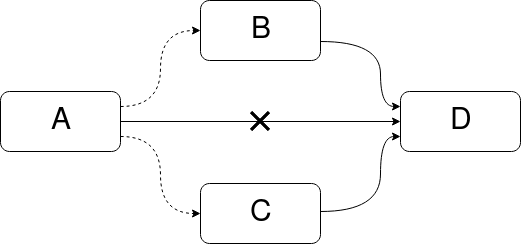
\includegraphics[height=4.5cm]{img/contetion-insertion}
    \caption{Condição de corrida durante inserção de nós}
    \label{figure-contention-insertion}
\end{figure}

Semelhantemente, para remoção de nós, se uma thread tentar remover um nó B e outra thread um nó C, ambos os nós ligados entre os nós A e D, os ponteiros dos nós A e B serão atualizados, o que resulta em apenas uma remoção, do nó B. Esse cenário está ilustrado na figura \ref{figure-contention-removal}.

\begin{figure}[htbp]
    \centering
    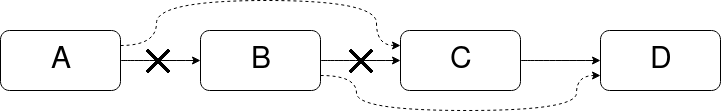
\includegraphics[height=2cm]{img/contetion-removal}
    \caption{Condição de corrida durante remoção de nós}
    \label{figure-contention-removal}
\end{figure}

\section{Evoluindo a implementação de uma lista ligada}\label{section-impl-evolution}

O uso de uma trava para garantir exclusão mútua durante essas duas atualizações (região crítica) é suficiente para tornar a operação segura para threads. Contudo, travas nas operações de inserção e remoção tornarão as operações totalmente seriais. Para evitar isso, é necessário definir as regiões críticas de maneira mais granular. Isso pode ser feito reduzindo as regiões críticas para as operações apenas nos nós específicos que se quer modificar. Assim, duas threads podem realizar modificações paralelamente em partes distintas da lista.

Para que isso seja possível, é necessário uma trava para cada nó e cada thread precisa realizar os travamentos em ordem, num processo chamado de \textit{lock coupling}: com exceção do primeiro nó, as travas só devem ser liberadas quando já se adquiriu a trava do nó seguinte. Assim as threads podem percorrer a lista com segurança, concorrentemente.

Ainda assim, pode haver bastante contenção de travas, em cenários em que há muitas threads percorrendo a lista. Além disso, apesar de ser possível realizar modificações paralelas na lista, uma thread modificando a lista impede que outras threads percorram o nó a ser modificado enquanto esse nó está travado. O paralelismo só é possível quando o segundo nó a ser modificado é anterior ao primeiro. Para alcançar paralelismo de busca e modificação independente da orden dos nós, outras abordagens são necessárias.

Uma abordagem útil para esse objetivo é a sincronização otimista: inicialmente a busca dos nós acontece sem travamento, e assim sem bloqueio. Ao encontrar o nó desejado, o nó é bloqueado e ocorre uma checagem de sua validade. Se durante a busca sem travamentos o nó foi removido, então a busca é reiniciada. Como esse tipo de conflito de sincronização é raro \cite{herlihy2011art}, essa abordagem pode ser muito eficiente. É necessário, contudo, que os nós removidos da lista não sejam removidos da memória. Ou seja, que ainda seja possível utilizar seus ponteiros para os nós seguintes, eventualmente encontrando o nó que se deseja, para verificar sua validade. Esse detalhe de implementação é trivial para linguagens com coletores automáticos de lixo.

Apesar de raro, ainda é possível em uma abordagem otimista que uma thread seja impedida infinitamente por outras operações, tendo que recomeçar a busca todas as vezes. Além disso, essa abordagem pode ser considerada indesejável em cenários que a operação de busca é muito mais comum do que a de inserção ou a de remoção \cite{herlihy2011art}, uma vez que toda operação de busca precisa utilizar as travas para realizer a checagem de validade dos nó encontrados.

\begin{figure}[htbp]
    \centering
        \begin{tabular}{ c | c | c | c | }
            \cline{2-4}
            & \texttt{insert} & \texttt{remove} & \texttt{contains} \\ \hline
            \multicolumn{1}{ | c | }{ \textit{coarse-grained} } & blocking & blocking & blocking \\ \hline
            \multicolumn{1}{ | c | }{ \textit{fine-grained} } & blocking & blocking & blocking \\ \hline
            \multicolumn{1}{ | c | }{ \textit{optimistic} } & blocking & blocking & blocking \\ \hline
            \multicolumn{1}{ | c | }{ \textit{lazy} } & blocking & blocking & wait-free \\ \hline
            \multicolumn{1}{ | c | }{ \textit{lock-free} } & lock-free & lock-free & wait-free \\ \hline
        \end{tabular}
    \caption{Comparação entre as operações das implementações}
    \label{figure-comparative-table}
\end{figure}

O próximo passo no processo de evolução seria justamente tornar a operação de busca \textit{wait-free}, ou seja, sem espera. Uma forma de alcançar esse objetivo é utilizar-se de um outro conceito: remoção lógica. A remoção lógica de um nó da lista se dá marcando o nó, sem alteração do ponteiro do nó anterior. Ou seja, o nó permanece ``fisicamente'' na lista, mas é considerado como removido.

Essa abordagem pode ser chamada de sincronização preguiçosa. Nessa abordagem, a operação de validação de nó não precisa percorrer toda a lista com o nó bloqueado, apenas checar se o nó e seu predecessor não estão marcados, e se o predecessor ainda aponta para o nó desejado. Dessa forma, as operações de inserção e remoção só precisam percorrer a lista novamente (recomeçando a operação) se o nó em questão não for mais válido.

Na figura \ref{figure-comparative-table} é apresentada uma comparação entre as operações das implementações, em termos de suas condições de progresso.

\section{Além de simples listas}

A implementação de listas ligadas não-bloqueantes e seguras para threads pode não parecer relevante em si mesma, uma vez que listas ligadas são estruturas simples, e é comum a necessidade de estruturas de dados mais complexas. Entretanto, é possível construir estruturas de dados mais complexas, como tabelas hash \cite{duarte2016concurrent}, conjuntos ordenados, skiplists \cite{herlihy2011art}, pilhas e filas de prioridade a partir de listas ligadas.

\chapter{Implementação em Haskell}\label{chapter-implementation}

As implementações desse trabalho podem fazer uso de travamento, \textit{compare-and-swap} e memória transacional.

Um ponto interessante da implementação é que para fazer uso das estruturas de sincronização (\texttt{MVar}s, \texttt{TVar}s \texttt{IORef}s), é necessário operar sobre a monad \texttt{IO}. Isso se deve ao fato de que as operações sobre essa implementação têm necessariamente efeitos colaterais.

Isso a tem desvantagem de que a implementação apresentada não é interoperável com as listas ordinárias (``nativas'') de Haskell. Portanto, para usar essa implementação em uma aplicação existente, o usuário terá que realizar modificações profundas. Casamento de padrões, por exemplo, não é factível para essa implementação.

Uma vantagem da implementação em Haskell, assim como acontece com outras linguagens com coleta automática de lixo, é que a remoção de um item da lista não implica na invalidação imediata do conteúdo da memória utilizada pelo item. Ou seja, o ponteiro para o próximo nó continua válido. Por isso, é possível alcançar um item que está na lista tendo passado por um que não está (como será mostrado na seção \ref{section-optimistic-implementation}).

Em todas as implementações, dois nós ``sentilenas'' serão usados para facilitar os algoritmos: o nós ``cabeça'' (\textit{head}) e o nó final (\textit{null}). Naturalmente, tais nós não influenciam na dimensão da lista.

\section{Coarse-grained}

A  implementação coarse-grained precisa somente de uma trava global. Em Haskell, isso significa apenas um \texttt{MVar} contendo a lista. Porém, para melhor comparação entre as implementações, um \texttt{IORef} será usado entre os nós. As definições dos tipos básicos dessa implementação estão representadas na Figura \ref{coarse-types}.

\begin{code}{coarse-types}{Tipos básicos da implementação Coarse-grained}
type Pointer a = IORef (List a)
data List a = Node { val :: a, next :: Pointer a }
    | Null
    | Head { next :: Pointer a }
    deriving Eq

newtype CoarseGrainedList a = CoarseGrainedList (MVar (Pointer a))
\end{code}

Para adicionar um item à lista, basta obter a trava global, percorrer a lista à procura da posição correta para o novo item, atualizar os ponteiros necessários e liberar a trava. Para evitar que exceções lançadas pelas threads que possuem a trava as impeçam de liberar as travas, causando \textit{starvation} nas demais threads, a função segura para exceções \texttt{withMVar} é utilizada, conforme pode-se observar na figura \ref{coarse-add}.

\begin{code}{coarse-add}{Função de inserção da implementação Coarse-grained}
add :: (Ord a) => (CoarseGrainedList a) -> a -> IO ()
add (CoarseGrainedList mvar) x =
    let
        go prevPtr = do
            prevNode <- readIORef prevPtr

            let currPtr = next prevNode
            currNode <- readIORef currPtr

            let newNode = Node { val = x, next = currPtr }
            newPtr <- newIORef newNode

            case currNode of
                Null -> updateNextPointer prevPtr newPtr
                Node { val = y } ->
                    if x <= y then updateNextPointer prevPtr newPtr
                    else go currPtr
                _ -> go currPtr

    in withMVar mvar go
\end{code}

A operação de remoção é bastante semelhante à de inserção. A diferença, como pode ser visto na figura \ref{coarse-remove}, é que o ponteiro do elemento a ser atualizado não é alterado para apontar para o novo elemento, mas para o seguinte ao que se quer remover.

\begin{code}{coarse-remove}{Função de remoção da implementação Coarse-grained}
remove :: (Eq a) => (CoarseGrainedList a) -> a -> IO Bool
remove (CoarseGrainedList mvar) x =
    let
        go prevPtr = do
            prevNode <- readIORef prevPtr

            let currPtr = next prevNode
            currNode <- readIORef currPtr

            case currNode of
                Null -> return False
                Node { val = y, next = nextPtr } ->
                    if x == y then updateNextPointer prevPtr nextPtr >> return True
                    else go currPtr
                _ -> go currPtr

    in withMVar mvar go
\end{code}

Nas duas funções apresentadas uma terceira função é usada, \texttt{updateNextPointer}, que é responsável pela alteração do ponteiros propriamente dita (figura \ref{coarse-update-pointer}). Naturalmente, não há necessidade de que essa operação seja atômica, uma vez que sempre haverá no máximo uma thread alterando ponteiros por vez, havendo a tava global.

\begin{code}{coarse-update-pointer}{Função de atualização de ponteiro da implementação Coarse-grained}
updateNextPointer :: (Pointer a) -> (Pointer a) -> IO ()
updateNextPointer firstPtr newPtr = do
    node <- readIORef firstPtr
    writeIORef firstPtr (node { next = newPtr })
\end{code}

Finalmente, a operação de busca está representada na figura \ref{coarse-contains}. Sua execução consiste simplemente em percorrer a lista à procura do elemento com o valor determinado, retornando a condição se sua presença na lista. Como a iteração de uma thread que percorre livremente uma lista pode ser invalidada pelas execuções de outras threads que modificam a lista, a operação de busca nessa implementação deve obter a trava global também.

\begin{code}{coarse-contains}{Função de busca da implementação Coarse-grained}
contains :: (Eq a) => (CoarseGrainedList a) -> a -> IO Bool
contains (CoarseGrainedList mvar) x =
    let
        go prevPtr = do
            prevNode <- readIORef prevPtr

            case prevNode of
                Null -> return False
                Head { next = nextPtr } -> go nextPtr
                Node { val = y, next = nextPtr } ->
                    if x == y then return True
                    else go nextPtr

    in withMVar mvar go
\end{code}

\section{Fine-grained}

Para dar mais liberdade para as threads executarem, a implementação Fine-grained propõe que cada nó tenha uma trava, ao invés de toda a lista ser controlada por uma trava global. Assim, diferentes threads podem percorrer diferentes partes da lista simultaneamente.

\begin{code}{fine-types}{Tipos básicos da implementação Fine-grained}
type Pointer a = IORef (MVar (List a))
newtype FineGrainedList a = FineGrainedList (Pointer a)

data List a = Node { val :: a, next :: Pointer a }
    | Null
    | Head { next :: Pointer a }
    deriving Eq
\end{code}

A figura \ref{fine-types} representa os tipos básicos da implementação Fine-grained. Dela pode-se perceber a mudança da trava global para uma trava em cada item, ``contida'' nos \texttt{IORef}s. Essa diferença influencia no modo de percorrer a lista. Para reduzir a complexidade de código, essa implementação abre mão da segurança contra exceções.

As figuras \ref{fine-add}, \ref{fine-remove} e \ref{fine-contains} mostram, respectivamente, as funções de inserção, remoção e busca da implementação Fine-grained.

\begin{code}{fine-add}{Função de inserção da implementação Fine-grained}
add :: (Eq a, Ord a) => FineGrainedList a -> a -> IO ()
add (FineGrainedList headPtr) x =
    let
        go prevMVar prevNode = do
            let currPtr = next prevNode
            currMVar <- readIORef currPtr
            currNode <- takeMVar currMVar
            case currNode of
                Node { val = y } ->
                    if (x > y) then do
                        putMVar prevMVar prevNode
                        go currMVar currNode
                    else do
                        let newNode = Node { val = x, next = currPtr }
                        newPtr <- newIORef =<< newMVar newNode
                        putMVar prevMVar (prevNode { next = newPtr })
                        putMVar currMVar currNode
                Null -> do
                    let newNode = Node { val = x, next = currPtr }
                    newPtr <- newIORef =<< newMVar newNode
                    putMVar prevMVar (prevNode { next = newPtr })
                    putMVar currMVar currNode
    in do
        headMVar <- readIORef headPtr
        headNode <- takeMVar headMVar
        go headMVar headNode
\end{code}

É fácil perceber o aumento da complexidade do código, por exemplo, ao notar que é necessário cobrir todas as possíveis ramificações da execução desbloqueando as travas, para não permitir que alguma permaneça travada indeterminadamente.

\begin{code}{fine-remove}{Função de remoção da implementação Fine-grained}
remove :: (Eq a, Ord a) => FineGrainedList a -> a -> IO Bool
remove (FineGrainedList headPtr) x =
    let
        go prevMVar prevNode = do
            let currPtr = next prevNode
            currMVar <- readIORef currPtr
            currNode <- takeMVar currMVar
            case currNode of
                Node { val = y } ->
                    if (x < y) then do
                        putMVar currMVar currNode
                        putMVar prevMVar prevNode
                        return False
                    else if (x > y) then do
                        putMVar prevMVar prevNode
                        go currMVar currNode
                    else do
                        putMVar currMVar currNode
                        putMVar prevMVar (prevNode { next = next currNode })
                        return True
                Null -> do
                    putMVar prevMVar prevNode
                    putMVar currMVar currNode
                    return False
    in do
        headMVar <- readIORef headPtr
        headNode <- takeMVar headMVar
        go headMVar headNode
\end{code}

As funções da implementação Fine-grained, assim como no caso da implementação Coarse-grained, são muito semelhantes. Isso porque todas precisam percorrer a lista e para percorrer a lista as travas precisam ser obtidas, e a atualização de ponteiros pode ser feita sem a necessidade de qualquer complexidade adicional, pois no momento que uma thread já adquiriu as travas, a atualização será necessariamente \textit{thread-safe}.

\begin{code}{fine-contains}{Função de busca da implementação Fine-grained}
contains :: Eq a => FineGrainedList a -> a -> IO Bool
contains (FineGrainedList headPtr) x =
    let
        go prevMVar prevNode = do
            let currPtr = next prevNode
            currMVar <- readIORef currPtr
            currNode <- takeMVar currMVar
            case currNode of
                Node { val = y } ->
                    if (x == y)
                    then do
                        putMVar prevMVar prevNode
                        putMVar currMVar currNode
                        return True
                    else do
                        putMVar prevMVar prevNode
                        go currMVar currNode
                Null -> do
                    putMVar prevMVar prevNode
                    putMVar currMVar currNode
                    return False
    in do
        headMVar <- readIORef headPtr
        headNode <- takeMVar headMVar
        go headMVar headNode
\end{code}

Como visto na seção \ref{section-impl-evolution}, o próximo passo é tornar a iteração pela lista menos custosa, removendo a necessidade de obter as travas de cada item.

\section{Optimistic}\label{section-optimistic-implementation}

Para que seja possível percorrer a lista sem obter as travas, os items com seus ponteiros para os próximos items não devem estar ``contidos'' em \texttt{MVar}s. Por isso, tuplas são utilizadas, para que estejam acessíveis, simultaneamente, item e trava (figura \ref{optimistic-types}).

\begin{code}{optimistic-types}{Tipos básicos da implementação Optimistic}
type Pointer a = IORef (List a, MVar ())
newtype OptimisticList a = OptimisticList (Pointer a)

data List a = Node { val :: a, next :: Pointer a }
    | Null
    | Head { next :: Pointer a }
    deriving Eq
\end{code}

A função de iteração está representada na figura \ref{optimistic-search}. Pode-se ver que as travas não são utilizadas, portanto a função não é segura para threads e portanto sua resposta pode ser inválida.

\begin{code}{optimistic-search}{Função de iteração da implementação Optimistic}
searchUnsafely :: Ord a => Pointer a -> a -> IO (PointerAndData a, PointerAndData a)
searchUnsafely prevPtr x = do
    (prevNode, prevMVar) <- readIORef prevPtr
    let currPtr = next prevNode
    (currNode, currMVar) <- readIORef currPtr

    let prevStuff = (prevPtr, prevMVar)
    let currStuff = (currPtr, currMVar)

    case currNode of
        Null -> return (prevStuff, currStuff)
        Node { val = y } -> do
            if y < x then searchUnsafely currPtr x
            else return (prevStuff, currStuff)
\end{code}

Por isso, se faz necessário uma função de validação, representada na figura \ref{optimistic-validate}. A função de validação verifica se o nó em questão é alcançável pelo nó cabeça. Essa verificação é necessária porque o nó pode já ter sido removido da lista. Um nó é alcançável se seu nó anterior ainda é alcançável e ainda aponta para o nó em questão. Claramente, as travas do nó em questão e do anterior precisam ser adquiridas para a validação.

\begin{code}{optimistic-validate}{Função de validação da implementação Optimistic}
validate :: Ord a => (Pointer a) -> (Pointer a) -> (List a) -> (Pointer a) -> IO Bool
validate headPtr prevPtr prevNode currPtr = go headPtr
    where
        go nodePtr = do
            (node, _) <- readIORef nodePtr

            case prevNode of
                Head { next = nextPtr } -> do
                    return $ nodePtr == prevPtr && nextPtr == currPtr
                Node { val = x, next = nextPtr } -> do
                    case node of
                        Null -> return False
                        Head { next = nextNodePtr } -> go nextNodePtr
                        Node { val = y, next = nextNodePtr } -> do
                            if  y > x then return False
                            else do
                                if nodePtr == prevPtr
                                then return $ nextPtr == currPtr
                                else go nextNodePtr
\end{code}

As figuras \ref{optimistic-add}, \ref{optimistic-remove} e \ref{optimistic-contains} representam, respectivamente, as operações de inserção, remoção e busca da implementação Optimistic. As estruturas dessas funções são muito semelhantes: a iteração insegura à procura pelo elemento em questão, bloqueio das travas do nó e do seu anterior, validação e a modificação determinada.

\begin{code}{optimistic-add}{Função de inserção da implementação Optimistic}
add :: (Eq a, Ord a) => OptimisticList a -> a -> IO ()
add list@(OptimisticList headPtr) x = do
    (prevStuff, currStuff) <- searchUnsafely headPtr x
    let (prevPtr, prevMVar) = prevStuff
    let (currPtr, currMVar) = currStuff

    let
        insert prevNode = do
            let newNode = Node x currPtr
            newPtr <- newIORef =<< ((,) newNode) <$> newMVar ()
            let newPredNode = prevNode { next = newPtr }
            writeIORef prevPtr (newPredNode, prevMVar)

        validationAndInsertion = do
            (prevNode, _) <- readIORef prevPtr
            (currNode, _) <- readIORef currPtr

            isValid <- validate headPtr prevPtr prevNode currPtr
            when isValid $ insert prevNode
            return isValid

    maybeSuccessful <- bracket_
        (mapM_ takeMVar [prevMVar, currMVar])
        (mapM_ (flip putMVar ()) [currMVar, prevMVar])
        validationAndInsertion

    if maybeSuccessful then return ()
    else add list x
\end{code}

Como o nó em questão pode já não ser mais válido, pode ser necessário, nesses casos, recomeçar a operação. Isso pode ser visto ao fim de cada função.

\begin{code}{optimistic-remove}{Função de remoção da implementação Optimistic}
remove :: (Eq a, Ord a) => OptimisticList a -> a -> IO Bool
remove list@(OptimisticList headPtr) x = do
    (prevStuff, currStuff) <- searchUnsafely headPtr x
    let (prevPtr, prevMVar) = prevStuff
    let (currPtr, currMVar) = currStuff

    let
        delete prevNode currNode = do
            let newPredNode = prevNode { next = next currNode }
            writeIORef prevPtr (newPredNode, prevMVar)

        validationAndRemoval = do
            (prevNode, _) <- readIORef prevPtr
            (currNode, _) <- readIORef currPtr

            isValid <- validate headPtr prevPtr prevNode currPtr
            if not isValid then return Nothing
            else do
                canBeRemoved <- case currNode of
                    Node { val = y } ->
                        if y == x then do
                            delete prevNode currNode
                            return True
                        else return False
                    Null -> return False
                return $ Just canBeRemoved

    maybeSuccessful <- bracket_
        (mapM_ takeMVar [prevMVar, currMVar])
        (mapM_ (flip putMVar ()) [currMVar, prevMVar])
        validationAndRemoval

    maybe (remove list x) return maybeSuccessful
\end{code}

É interessante notar nessas funções o uso da função \texttt{bracket\_} de Haskell, que torna o processo seguro à exceções.

\begin{code}{optimistic-contains}{Função de busca da implementação Optimistic}
contains :: (Eq a, Ord a) => OptimisticList a -> a -> IO Bool
contains list@(OptimisticList headPtr) x = do
    (prevStuff, currStuff) <- searchUnsafely headPtr x
    let (prevPtr, prevMVar) = prevStuff
    let (currPtr, currMVar) = currStuff

    let
        validationAndCheck = do
            (prevNode, _) <- readIORef prevPtr
            (currNode, _) <- readIORef currPtr

            isValid <- validate headPtr prevPtr prevNode currPtr
            if not isValid then return Nothing
            else case currNode of
                Null -> return $ Just False
                Node { val = y } -> return . Just $ x == y

    maybeSuccessful <- bracket_
        (mapM_ takeMVar [prevMVar, currMVar])
        (mapM_ (flip putMVar ()) [prevMVar, currMVar])
        validationAndCheck

    maybe (contains list x) return maybeSuccessful
\end{code}

\section{Lazy}

Seguindo a seção \ref{section-impl-evolution}, o próximo passo na evolução das implementações é tornar a operação de busca menos custosa. Para isso, é feito uso de um mecanismo de remoção lógica, usando uma marcação. Os tipos básicos da implementação Lazy estão representados na figura \ref{lazy-types}.

\begin{code}{lazy-types}{Tipos básicos da implementação Lazy}
type Mark = IORef Bool
type Pointer a = IORef (List a, MVar (), Mark)
newtype LazyList a = LazyList (Pointer a)

data List a = Node { val :: a, next :: Pointer a }
    | Null
    | Head { next :: Pointer a }
    deriving Eq
\end{code}

A função de iteração é igual à da implementação Optimistic.

\begin{code}{lazy-search}{Função de iteração da implementação Lazy}
searchUnsafely :: Ord a => Pointer a -> a -> IO (PointerAndData a, PointerAndData a)
searchUnsafely prevPtr x = do
    (prevNode, prevMVar, prevMark) <- readIORef prevPtr
    let currPtr = next prevNode
    (currNode, currMVar, currMark) <- readIORef currPtr

    let prevStuff = (prevPtr, prevMVar)
    let currStuff = (currPtr, currMVar)

    case currNode of
        Null -> return (prevStuff, currStuff)
        Node { val = y } -> do
            if y < x then searchUnsafely currPtr x
            else return (prevStuff, currStuff)
\end{code}

Ao contrário da implementação Optimistic, a implementação Lazy tem uma função de validação que não precisa percorrer a lista para verificar se o nó em questão é alcançável. Basta checar se o nó em questão e o anterior não estão marcados e se o anterior ainda aponta para o nó em questão. Portanto, a verificação é, agora, em tempo constante.

Se algum dos nós está marcado, então foi removido logicamente. Se o anterior não aponta para o nó em questão, então outro nó foi inserido entre eles. Em qualquer caso, deve-se reiniar a operação.

\begin{code}{lazy-validation}{Função de validação da implementação Lazy}
validate :: Eq a => (List a) -> (Pointer a) -> Mark -> Mark -> IO Bool
validate prevNode currPtr prevMark currMark = do
    prevMarked <- readIORef prevMark
    currMarked <- readIORef currMark

    return $ (not prevMarked) && (not currMarked) && (next prevNode == currPtr)
\end{code}

Como a função de validação não percorre a lista, as operações de inserção e remoção só precisam percorrer uma única vez, caso não haja contenção.

As figuras \ref{lazy-add}, \ref{lazy-remove} e \ref{lazy-contains} representam, respectivamente, as operações de inserção, remoção e busca da implementação Lazy. As estruturas dessas funções seguem exatamente a mesmo estrutura da implementação Optimistic.

\begin{code}{lazy-add}{Função de inserção da implementação Lazy}
add :: (Eq a, Ord a) => LazyList a -> a -> IO ()
add list@(LazyList headPtr) x = do
    (prevStuff, currStuff) <- searchUnsafely headPtr x
    let (prevPtr, prevMVar) = prevStuff
    let (currPtr, currMVar) = currStuff

    let
        insert prevNode = do
            let newNode = Node x currPtr
            newPtr <- newIORef =<< ((,,) newNode) <$> newMVar () <*> newIORef False
            let newPredNode = prevNode { next = newPtr }
            atomicWriteIORef prevPtr =<< ((,,) newPredNode) <$> pure prevMVar <*> newIORef False

        validationAndInsertion = do
            (prevNode, _, prevMark) <- readIORef prevPtr
            (currNode, _, currMark) <- readIORef currPtr

            isValid <- validate prevNode currPtr prevMark currMark
            when isValid $ insert prevNode
            return isValid

    maybeSuccessfull <- bracket_
        (mapM_ takeMVar [prevMVar, currMVar])
        (mapM_ (flip putMVar ()) [currMVar, prevMVar])
        validationAndInsertion

    if maybeSuccessfull then return ()
    else add list x
\end{code}

Nota-se na implemetação das operações de inserção e remoção o uso da função \texttt{atomicWriteIORef}, que, sendo baseada na função \texttt{atomicModifyIORef}, garantem consistência sequencial. Isso é necessário porque nessa implementação a validação não percorre novamente a lista, e as possíveis reordenações dos processadores (como visto na seção \ref{subsection-atomicmodifyioref}) podem invalidar a lista.

A operação de remoção é feita em duas etapas: lógica e ``física'', nessa ordem. Dessa forma, a função de validação sempre observará a remoção lógica antes que os efeitos da remoção ``física'' sejam aplicados.

\begin{code}{lazy-remove}{Função de remoção da implementação Lazy}
remove :: (Eq a, Ord a) => LazyList a -> a -> IO Bool
remove list@(LazyList headPtr) x = do
    (prevStuff, currStuff) <- searchUnsafely headPtr x
    let (prevPtr, prevMVar) = prevStuff
    let (currPtr, currMVar) = currStuff

    let
        delete prevNode prevMark currNode currMark = do
            atomicWriteIORef currMark True
            let newPredNode = prevNode { next = next currNode }
            writeIORef prevPtr =<< ((,,) newPredNode) <$> pure prevMVar <*> pure prevMark

        validationAndRemoval = do
            (prevNode, _, prevMark) <- readIORef prevPtr
            (currNode, _, currMark) <- readIORef currPtr

            isValid <- validate prevNode currPtr prevMark currMark
            if not isValid then return Nothing
            else do
                canBeAdded <- case currNode of
                    Node { val = y } ->
                        if y == x then do
                            delete prevNode prevMark currNode currMark
                            return True
                        else return False
                    Null -> return False
                return $ Just canBeAdded

    maybeSuccessfull <- bracket_
        (mapM_ takeMVar [prevMVar, currMVar])
        (mapM_ (flip putMVar ()) [currMVar, prevMVar])
        validationAndRemoval

    maybe (remove list x) return maybeSuccessfull
\end{code}

A função de busca da implementação Lazy é \textit{wait-free}, pois não depende de qualquer maneira da execução de outras threads para progredir.

\begin{code}{lazy-contains}{Função de busca da implementação Lazy}
contains :: Ord a => LazyList a -> a -> IO Bool
contains list@(LazyList headPtr) x = do
    (headNode, _, _) <- readIORef headPtr
    maybeCurr <- findCurr (next headNode) x
    case maybeCurr of
        Nothing -> return False
        Just (currVal, currMark) -> do
            currMarked <- readIORef currMark
            return $ x == currVal && not currMarked
    where
        findCurr currPtr val = do
            (currNode, _, currMark) <- readIORef currPtr
            case currNode of
                Null -> return Nothing
                Node { val = y } ->
                    if y < x then findCurr (next currNode) val
                    else return $ Just (y, currMark)
\end{code}

\section{Lock-free}

O próximo passo na evolução das implementações é tornar as operações de inserção e remoção não-bloqueantes. Com isso, todas as operações serão \textit{lock-free}, mas não \textit{wait-free} (somente a operação de busca).

Semelhantemante à implementação Lazy, a implementação Lock-free faz uso do conceito de remoção lógica. Porém, como a nova implementação não pode conter travas, essa marcação deve estar contida no tipo de item da lista. Esse detalhe de implementação, assim como os tipos básicos, estão representados na figura \ref{lockfree-types}.

\begin{code}{lockfree-types}{Tipos básicos da implementação Lock-free}
type Pointer a = IORef (List a)
newtype LockFreeList a = LockFreeList (Pointer a)

data List a = Node { val :: a, next :: Pointer a }
    | DelNode { next :: Pointer a }
    | Null
    | Head { next :: Pointer a }
    deriving Eq
\end{code}

Essa abordagem pode ser comparada com o uso da classe \texttt{AtomicMarkableReference}, da linguagem Java, que oferece uma forma de alterar o valor de um ponteiro e marcá-lo atomicamente. Isso é possível fazendo uso dos bits menos significativos dos ponteiros, o que não interfere no endereço, já que os ponteiros são alinhados na memória \cite{herlihy2011art}.

Usando a função \texttt{atomicModifyIORef}, é fácil construir uma função de \textit{compare-and-swap}, que, atomicamente, altera o valor do \texttt{IORef} somente se o mesmo já não tier sido alterado tendo um determinado valor como referência. Essa função está representada na figura \ref{lockfree-cas}.

\begin{code}{lockfree-cas}{Função auxiliar de compare-and-swap}
atomCAS :: Eq a => IORef a -> a -> a -> IO Bool
atomCAS ptr old new =
    atomicModifyIORef ptr $ \curr ->
        if curr == old then (new, True)
        else (curr, False)
\end{code}

Na implementação Lazy, as únicas funções que não fazem uso de travas são as de validação e de iteração, que não modificam a lista. Por isso, a removação lógica imediatamente anterior à remoção ``física'' é suficiente. Já não é o caso para a implementação Lock-free, que pode ter várias operações que modificam a lista sendo executas simultaneamente, sem travas.

Portanto, na implementação Lock-free, a operação de remoção, representada na figura \ref{lockfree-remove}, apenas realiza a remoção lógica.

\begin{code}{lockfree-remove}{Função de remoção da implementação Lock-free}
remove :: (Eq a, Ord a) => LockFreeList a -> a -> IO Bool
remove list x = do
    (prevPtr, prevNode, currPtr, currNode, found) <- window list x

    if not found then return False
    else do
        -- if element is found, it is not tail
        let nextPtr = next currNode

        let markedCurrNode = DelNode { next = nextPtr }
        b <- atomCAS currPtr currNode markedCurrNode
        if not b then remove list x
        else do
            let newPrevNode = prevNode { next = nextPtr }
            atomCAS prevPtr prevNode newPrevNode
            return True
\end{code}

Assim como a operação de remoção, a operação de inserção, representada na figura \ref{lockfree-add}, é reiniciada todas as vezes que a alteração não for possível por motivo de alteração do elemento em questão ou seu anterior.

\begin{code}{lockfree-add}{Função de inserção da implementação Lock-free}
add :: (Eq a, Ord a) => LockFreeList a -> a -> IO ()
add list x = do
    (prevPtr, prevNode, currPtr, currNode, _) <- window list x

    let newNode = Node x currPtr
    newPtr <- newIORef newNode
    let newPrevNode = prevNode { next = newPtr }

    b <- atomCAS prevPtr prevNode newPrevNode
    if not b then add list x
    else return ()
\end{code}

É a função de iteração (figura \ref{lockfree-search}) que realiza as remoções ``físicas''. Durante a iteração, quando um elemento marcado é alcançado, o seu elemento anterior é analisado. Se o elemento anterior também estiver marcado, toda a iteração é reiniciada. Se não estiver marcado, ele é alterado para apontar para o próximo do elemento a ser removido. Se a alteração falhar (por motivo do ponteiro já ter sido alterado), toda a iteração é reiniciada.

\begin{code}{lockfree-search}{Função de iteração da implementação Lock-free}
window :: Ord a => LockFreeList a -> a -> IO (Pointer a, List a, Pointer a, List a, Bool)
window (LockFreeList head) x =
    let
        go prevPtr = do
            prevNode <- readIORef prevPtr
            let currPtr = next prevNode
            currNode <- readIORef currPtr

            case currNode of
                DelNode { next = nextPtr } -> do
                    case prevNode of
                        DelNode {} -> go head
                        Head {} -> do
                            let newPrevNode = Head nextPtr
                            b <- atomCAS prevPtr prevNode newPrevNode
                            if not b then go head
                            else go currPtr
                        Node {} -> do
                            let newPrevNode = prevNode { next = nextPtr }
                            b <- atomCAS prevPtr prevNode newPrevNode
                            if not b then go head
                            else go currPtr
                Node { val = y, next = nextPtr } -> do
                    if y == x then do
                        return (prevPtr, prevNode, currPtr, currNode, True)
                    else if y > x then do
                        return (prevPtr, prevNode, currPtr, currNode, False)
                    else go currPtr
                Null -> return (prevPtr, prevNode, currPtr, currNode, False)
    in go head
\end{code}

Assim como na implementação Lazy, a função de busca da implementação Lock-free, representada na figura \ref{lockfree-contains}, é \textit{wait-free}.

\begin{code}{lockfree-contains}{Função de busca da implementação Lock-free}
contains :: (Eq a, Ord a) => LockFreeList a -> a -> IO Bool
contains (LockFreeList headPtr) x =
    let
        go prevPtr = do
            prevNode <- readIORef prevPtr
            let currPtr = next prevNode
            currNode <- readIORef currPtr

            case currNode of
                Null -> return False
                DelNode { next = nextPtr } -> go nextPtr
                Node { val = y, next = nextPtr } -> do
                    if y == x then return True
                    else if y > x then return False
                    else go currPtr
    in go headPtr
\end{code}

\section{STM}

Para efeito de comparação, há também uma implementação semelhante à Lockfree, porém construída utilizando memória transacional. Para não incorrer em um volume excessivo de conflitos de transações, pequenas transações serão realizadas, diminuindo as possibilidades de conflito.

\begin{code}{stm-types}{Tipos básicos da implementação STM}
type Pointer a = TVar (List a)
newtype StmList a = StmList (Pointer a)

data List a = Node { val :: a, next :: Pointer a }
    | DelNode { next :: Pointer a }
    | Head { next :: Pointer a }
    | Null
    deriving Eq
\end{code}

Por usar a biblioteca padrão de memória transacional do GHC (\texttt{stm}), o tipo \texttt{TVar} é utilizado, ao invés de \texttt{MVar}s. Nota-se o uso de remoção lógica.

\begin{code}{stm-search}{Função de iteração da implementação STM}
searchAndExecute ::
    (Eq a, Ord a)
    => StmList a
    -> a
    -> (Pointer a -> List a -> Pointer a -> List a -> Bool -> STM (IO Bool))
    -> IO Bool
searchAndExecute (StmList head) x function =
    let
        go prevPtr = runStmTransactions $ do
            prevNode <- readTVar prevPtr
            let curPtr = next prevNode
            curNode <- readTVar curPtr

            case curNode of
                DelNode { next = nextNode } ->
                    case prevNode of
                        DelNode {} -> return (go head)
                        Head {} -> do
                            writeTVar prevPtr $ Head nextNode
                            return (go prevPtr)
                        Node { val = y } -> do
                            writeTVar prevPtr $ Node y nextNode
                            return (go prevPtr)
                Null -> function prevPtr prevNode curPtr curNode False
                Node { val = y, next = nextNode } -> do
                    if x == y then function prevPtr prevNode curPtr curNode True
                    else if y > x then function prevPtr prevNode curPtr curNode False
                    else return (go curPtr)
    in go head

runStmTransactions :: STM (IO a) -> IO a
runStmTransactions stm = do
    io <- atomically stm
    io
\end{code}

Como já explicado, a implementação STM faz uso de pequenas transações para evitar conflitos. A função de iteração da implementação STM está representada na figura \ref{stm-search}, onde essa propriedade pode ser observada.

Cada passo da iteração representa uma transação, que ``carrega'' uma ação monádica \texttt{IO}. Essa ação é necessária para criar as próximas transações. A função \texttt{runStmTransactions} (figura \ref{stm-search}) executa cada transação e sua ação \texttt{IO}. Nessa ação pode haver outra chamada à \texttt{runStmTransactions}, para a próxima iteração.

\begin{code}{stm-operations}{Funções de inserção, remoação e busca da implementação STM}
add :: (Eq a, Ord a) => (StmList a) -> a -> IO ()
add list x = do
    searchAndExecute list x $ \prevPtr prevNode curPtr curNode _ -> do
        newPtr <- newTVar $ Node x curPtr
        writeTVar prevPtr $ prevNode { next = newPtr }
        return $ return True
    return ()

remove :: (Eq a, Ord a) => (StmList a) -> a -> IO Bool
remove list x = searchAndExecute list x $ \prevPtr prevNode curPtr curNode itemFound -> do
    if not itemFound then return $ return False
    else do
        writeTVar curPtr (DelNode $ next curNode)
        return $ return True

contains :: (Eq a, Ord a) => (StmList a) -> a -> IO Bool
contains list x = searchAndExecute list x $ \_ _ _ _ itemFound -> return $ return itemFound
\end{code}

Na figura \ref{stm-operations} estão representadas as operações de inserção, remoção e busca. Suas implementações são triviais, fazendo uso da função de iteração e atualizando os ponteiros necessários.

\section{Interface unificada}

Para facilitar o uso das implementações, bem como a substituição de uma implemetação por outra em uma aplicação (e os testes desse trabalho), pode ser utilizada uma interface. Na figura \ref{thread-safe-class} está representada essa interface. Como ela é paramétrica em dois tipos (a implementação e o tipo dos elementos), é necessário fazer uso da extensão \texttt{MultiParamTypeclasses}, do GHC.

\begin{code}{thread-safe-class}{Interface para as implementações}
{-# LANGUAGE MultiParamTypeClasses #-}

module ThreadSafeList
    ( ThreadSafeList
    , newEmptyList
    , toPureList
    , add
    , remove
    , contains
    ) where

class ThreadSafeList l a where
    newEmptyList :: IO (l a)
    toPureList :: l a -> IO [a]
    add :: l a -> a -> IO ()
    remove :: l a -> a -> IO Bool
    contains :: l a -> a -> IO Bool
\end{code}

Para que seja possível escolher dinamicamente uma implementação, é necessário um tipo que englobe todas as implementações, e esse tipo está representado na figura \ref{thread-safe-data}. Essa funcionalidade requer a extensão \texttt{ExistentialQuantification} do GHC.

\begin{code}{thread-safe-data}{Tipo que engloba todas as implementações}
{-# LANGUAGE ExistentialQuantification #-}

import qualified ThreadSafeList as TSL
import qualified CoarseGrained as CG
import qualified FineGrained as FG
import qualified Optimistic as O
import qualified Lazy as L
import qualified LockFree as LF
import qualified STM as STM

data ThreadSafeList a =
    forall l. TSL.ThreadSafeList l a => ThreadSafeList (l a)

data ListType = CoarseGrained
    | FineGrained
    | Optimistic
    | Lazy
    | LockFree
    | STM
    deriving (Show, Bounded, Enum)

newEmptyList :: Ord a => ListType -> IO (ThreadSafeList a)
newEmptyList CoarseGrained = fmap ThreadSafeList CG.newEmptyList
newEmptyList FineGrained = fmap ThreadSafeList FG.newEmptyList
newEmptyList Optimistic = fmap ThreadSafeList O.newEmptyList
newEmptyList Lazy = fmap ThreadSafeList L.newEmptyList
newEmptyList LockFree = fmap ThreadSafeList LF.newEmptyList
newEmptyList STM = fmap ThreadSafeList STM.newEmptyList

add :: ThreadSafeList a -> a -> IO ()
add (ThreadSafeList l) x = TSL.add l x

remove :: ThreadSafeList a -> a -> IO Bool
remove (ThreadSafeList l) x = TSL.remove l x

contains :: ThreadSafeList a -> a -> IO Bool
contains (ThreadSafeList l) x = TSL.contains l x
\end{code}

\chapter{Avaliando o desempenho}\label{chapter-analysis}

\section{Metodologia}

Os testes foram realizados de modo a mensurar o desempenho absoluto de cada implementação, em um multiprocessador de 4 núcleos (Intel Core i5-3317U 1.70GHz com 6GB de memória RAM). A versão do GHC utilizada foi a 8.0.2 e o sistema operacional foi o Linux, na versão 4.14.3.

Para obter resultados estatisticamente relevantes, o arcabouço de \textit{benchmarking} Criterion (disponível no Hackage \footnote{https://hackage.haskell.org/package/criterion}) foi utilizado. O Criterion é robusto o suficiente para descartar o ruído estatístico proveniente na coleta de lixo de memória ou do escalonamento do sistema operacional, por exemplo \cite{lima2016haskell}. Regressão linear é utilizada pelo arcabouço para estimar o tempo de uma execução, a partir da mensuração de várias sequências de execuções.

Dois benchmarks foram criados, um de alta contenção e outro simulando um cenário mais realístico. O benchmark de alta contenção consiste em várias threads tentando inserir o número 42 em umas lista de números gerados aleatoriamente entre 0 e 100. Enquanto isso, uma thread tenta inserir o número 41 e outra remover o número 41. O número de threads total é igual ao número de núcleos do multiprocessador, e cada thread tenta realizar sua operação 10000 vezes.

O benchmark realístico consiste em várias threads (tantas quanto o número de núcleos do processador) realizando operações geradas aleatoriamente em uma lista gerada aleatoriamente. As operações são geradas de acordo com a seguinte proporção: 20\% são inserções, 10\% são remoções e 70\% são buscas. Esses números representam um cenário realístico \cite{sulzmann2009comparing}.

\section{Resultados}

Os benchmarks foram analisados em três ambientes: coletor de lixo paralelo (configuração padrão do GHC para múltiplas threads), coletor de lixo sequencial e coletor de lixo com o uso da extensão \texttt{BangPatterns}, que força a avalição de determinadas expressões até o primeiro construror (\textit{WHNF}).

É de se imaginar que a implementação sem travas é a mais eficiente, mas não se pode esquecer que a operação de \textit{compare-and-swap} também apresenta algum overhead.

\begin{center}
\begin{graph}{Benchmark de alta contenção com GC paralelo}{bench-high-contention}
\begin{bchart}[step=3,max=16,unit=s,width=.9\textwidth]
    \bcbar[text=CoarseGrained]{4.79}
        \smallskip
    \bcbar[text=FineGrained]{3.18}
        \smallskip
    \bcbar[text=Optimistic]{6.98}
        \smallskip
    \bcbar[text=Lazy]{2.74}
        \smallskip
    \bcbar[text=LockFree]{2.60}
        \smallskip
    \bcbar[text=STM]{16.08}
    \bcxlabel{Segundos}
\end{bchart}
\end{graph}
\end{center}

A figura \ref{bench-high-contention} contém um comparativo das implementações no cenário de alta contenção com o coletor de lixo paralelo. Destaca-se a performance precária da implementação STM, seguida da implementação Optimistic.

Uma possibilidade para o resultado da implementação Optimistic é a alta ocorrência de iteração sobre a lista (para validação, algo que as outras implementações não necessitam), e a operação de busca necessitar obter as travas.

\begin{center}
\begin{graph}{Benchmark de cenário realístico com GC paralelo}{bench-realistic}
\begin{bchart}[step=3,max=30,unit=s,width=.9\textwidth]
    \bcbar[text=CoarseGrained]{29.31}
        \smallskip
    \bcbar[text=FineGrained]{9.28}
        \smallskip
    \bcbar[text=Optimistic]{8.93}
        \smallskip
    \bcbar[text=Lazy]{5.66}
        \smallskip
    \bcbar[text=LockFree]{5.77}
        \smallskip
    \bcbar[text=STM]{23.69}
    \bcxlabel{Segundos}
\end{bchart}
\end{graph}
\end{center}

No benchmark de cenário realístico, a implementação Optimistic se comporta de modo esperado. Novamente não é o caso da implementação STM. Apesar do uso de transações pequenas para evitar conflitos, essa implementação ainda apresenta um desempenho bastante precário.

Destaca-se neste cenário a implementação Lazy, que obteve o melhor resultado. A operação de busca \textit{wait-free} e a validação em tempo constante com certeza contribuem para esse resultado, dado o overhead que a implementação Lockfree possui como consequência da operação \textit{compare-and-swap}.

\begin{center}
\begin{graph}{Benchmark de alta conteção com GC sequencial}{bench-realistic-no-parallel-gc}
\begin{bchart}[step=3,max=12,unit=s,width=.9\textwidth]
    \bcbar[text=CoarseGrained]{4.49}
        \smallskip
    \bcbar[text=FineGrained]{3.15}
        \smallskip
    \bcbar[text=Optimistic]{7.70}
        \smallskip
    \bcbar[text=Lazy]{2.76}
        \smallskip
    \bcbar[text=LockFree]{2.61}
        \smallskip
    \bcbar[text=STM]{10.63}
    \bcxlabel{Segundos}
\end{bchart}
\end{graph}
\end{center}

Os benchmarks com coletor de lixo sequencial não mostraram grande diferença em relação aos benchmarks com coletor de lixo paralelo. Destaca-se, contudo, que algumas implementações foram mais eficientes com o coletor sequencial.

\begin{center}
\begin{graph}{Benchmark de cenário realístico com GC sequencial}{bench-realistic-no-parallel-gc}
\begin{bchart}[step=3,max=27,unit=s,width=.9\textwidth]
    \bcbar[text=CoarseGrained]{21.43}
        \smallskip
    \bcbar[text=FineGrained]{9.15}
        \smallskip
    \bcbar[text=Optimistic]{8.71}
        \smallskip
    \bcbar[text=Lazy]{5.32}
        \smallskip
    \bcbar[text=LockFree]{5.50}
        \smallskip
    \bcbar[text=STM]{25.13}
    \bcxlabel{Segundos}
\end{bchart}
\end{graph}
\end{center}

Para analisar parte do impacto da avaliação preguiçosa na eficiência das implementações, os benchmarks foram executados fazendo uso da extensão do \texttt{BangPatterns} do GHC. Não foi percebido, contudo, diferença nos resultados. Acredita-se que as implementações como foram feitas oferecem poucas oportunidades significativas para qualquer efeito negativo da avaliação preguiçosa.

\chapter{Conclusão}\label{chapter-conclusion}

Ao contrário do que já foi mostrado antes \cite{sulzmann2009comparing}, esse trabalho demonstra que nem sempre o uso de travas para sincronização é a melhor opção para encontrar o melhor desempenho possível para estruturas de dados seguras para threads, especialmente levando em consideração a complexidade de implementação. Porém, para os benchmarks analisados, não deixou de ser uma ótima opção, por não haver diferença realmente significativa nos casos em que não foi a implementação mais eficiente.

O uso de memória transacional para sincronização de operações de estruturas de dados se mostrou bastante ineficiente, sendo superado em vários casos por implementações inocentes usando travas.

\section{Trabalhos relacionados}

Existe alguma literatura sobre o tema desse trabalho, e interesse crescente, mas não muita. Newton et al \cite{newton2011intel} demonstraram a criação de estruturas de dados concorrentes utilizando trocas de mensagens.

Discolo et al \cite{discolo2006lock} e Duarte et al \cite{duarte2016concurrent} compararam de modo mais detalhado as diferenças de implementação e performance entre as versões com travas e usando memória transacional das estruturas de dados, respectivamente, filas e tabelas hash.

Semelhantemante a este trabalho, Sulzmann et al \cite{sulzmann2009comparing} demonstraram a difereça de implementações de listas ligadas não-bloqueantes, usando a operação \textit{compare-and-swap} e memória transacional.

Utilizando-se da linguagem Java, Herlihy et al \cite{herlihy2011art} também discorreram sobre possíveis implementações e evolução de implementações de listas seguras para threads.

Este trabalho é fortemente inspirado pelos trabalhos de Sulzmann et al e Herlihy et al.

\section{Trabalhos Futuros}

Há vários pontos de melhoria para esse trabalho, que poderão ser explorados futuramente. Primeiramente, análise de corretude das implementações. Isso é algo que Herlihy et al \cite{herlihy2011art} fazem para suas implementações em Java.

Além disso, análise profunda do comportamento do coletor de lixo do GHC. Dessa análise podem ser obtidas conclusões pertinentes que podem explicar o baixo desempenho de alguma implmentação.

Além a análide de coleta de lixo, também pode ser proveitoso realizar análise do comportamento das threads, o que pode ser feito com o uso da ferramenta ThreadScope \footnote{https://wiki.haskell.org/ThreadScope}.

Benchmarking usando aplicações reais em cenários reais (ao invés de \textit{realísticos}), para melhor averiguação do desempenho, é outro ponto sério de melhoria.

Além disso, seguindo trabalhos anteriores \cite{lima2016haskell}, há bastante interesse na análise do consumo de energia.

Por último, implementação de outras estruturas de dados, como tabelas hash e árvores.

\bibliographystyle{abbrv}
\bibliography{references}

\end{document}
